\documentclass[twoside,12pt]{article}
\newcommand{\tab}{\hspace*{2em}}
\usepackage{light}
\usepackage{subfigure}
\usepackage{graphicx}
\usepackage{amsmath}
\usepackage{verbatim}

\newcommand{\lr}{l_{right}}
\renewcommand{\ll}{l_{left}}

\newcommand{\card}[1]{\left|#1\right|}


%\hidesolutions
\showsolutions


\begin{document}

\problemset{5}{October 11, 2012}{Wednesday, October 10}
%In this problem set, we will use some notation not present in the textbook:
%\begin{itemize}
%\item  The $\oplus $ operator is the logical $\xor$ operator, so $A \oplus B$ is True  when $A$ is True and $B$ is False, or when  $B$ is True and $A$ is False, and $A \oplus B$ is False when $A$ and $B$ are both True or are both False. 
%\item The $\lnot$ operator is the NOT operator. $\lnot A$ is True when A is False, and 
%$\lnot A$ is False when A is True.
%\item The $\land$ is the logical AND operator.
%\item The $\lor$ is the logical OR operator.

%\item $A \iff B$ means $A$ iff $B$.\\
%\end{itemize}
%%%%%%%%%%%%%%%%%%%%%%%%%%%%%%%%%%%%%%%%%%%%%%%%%%%%%%%%%%%%%%%%%%%%%%%%%%%%%%%

\begin{problem}{9} For each graph in Figure 1, find an Euler tour (if one exists) or an Euler walk (if one exists and there is no Euler tour).

\begin{figure}[h]
\label{tentree}
\centerline{\includegraphics[scale=0.85]{ps5_fig1t.pdf}}
\caption{Graphs}
\end{figure}

\solution{
(a) has an Euler walk: c-a-b-c-d-b; it does not have an Euler tour.

(b) has an Euler walk: c-e-a-d-b-f-a-b-c-d-e-f; it does not have an Euler tour.

(c) has an Euler tour: a-c-b-h-i-a-b-i-c-g-h-d-g-f-e-c-d-e-h-a. 

}
\end{problem}  


%%%%%%%%%%%%%%%%%%%%%%%%%%%%%%%%%%%%%%%%%%%%%%%%%%%%%%%%%%%%%%%%%%%%%%%%%%%%%%%

\begin{comment}
\begin{problem}{10}
Complete binary trees with $N$ inputs and $N$ outputs, where $N=2^n$
for some $n\geq 0$, were described in class and the notes.  In this
problem we consider complete \emph{ternary} trees with $N$ inputs
and $N$ outputs, where $N=3^n$. The following figure shows a ternary
tree with 3 inputs and 3 outputs (i.e $N=3$, and $n=1$).

%\figure{!}{2in}{pset5-tentree}

\bparts \ppart{5} Find a closed-form expression for the diameter of the
$N$-input, $N$-output ternary tree.

\solution{ The diameter is $2 \log_3 N + 2$, or $2n + 2$. }

\ppart{5} Prove that your expression is correct using induction.
\textit{Hint:} Your induction hypothesis should prove an expression
for the length of a path from an input to the root node.\\

\solution{We proceed by induction on $n$.  Let $P(n)$ be the
proposition that, in a complete ternary tree with $N=3^n$ inputs and
outputs:
\begin{itemize}
\item the number of edges in the path from any input to the root node,
or from the root node to an output is $n + 1$, and
\item the diameter in the tree is $2n + 2$.
\end{itemize}

\textbf{Base case} ($n=0$): A complete ternary tree with $N=3^0=1$
input and $1$ output consists of those two input/output nodes plus a
single switch. The only path from the input to the root traverses
$1$ edge, which equals $n + 1 = 0 + 1$. Similarly, the only path
from the root to the output traverses $1$ edge. The only path from
the input to the output traverses 2 edges, which equals $2n + 2 = 0
+ 2$. Thus $P(0)$ is true.

\textbf{Inductive step.}  Now assume $P(n)$ for $n \geq 0$ in order
to prove $P(n+1)$.  A complete ternary tree $T_0$ with $3^{n+1}$
inputs and $3^{n+1}$ outputs is constructed from three complete
ternary trees $T_1, T_2, T_3$ with $3^n$ inputs and $3^n$ outputs by
connecting their root nodes to a single new root node $r_0$.

By the inductive hypothesis, the length of a path from an input in
$T_1$ to its root $r_1$ is $n + 1$.  This root node is connected to
the new root $r_0$ by two edges $(r_0,r_1)$ and $(r_1,r_0)$.  Thus
the path from an input in $T_1$ to $r_0$ traverses $(n + 1) + 1$
edges, as required.  This same argument applies to the trees $T_2$
and $T_3$.

If an input and an output belong to $T_1$ then, by the inductive
hypothesis, the path between them traverses $2n + 2$ edges. For an
input and output in different subtrees, say $T_1$ and $T_2$, the
shortest path between them consists of the path from the input to
$r_1$, the edges $(r_1,r_0)$ and $(r_0,r_2)$, and the path from
$r_2$ to the output. This path traverses $(n + 1) + 2 + (n + 1) =
2(n + 1) + 2$ edges, as required. Thus the maximum distance from any
input to any output is $2(n+1) + 2$. Since such a path between nodes
in different subtrees will always exist, as the tree is connected,
this will be the minimum diameter as well, and so the diameter must
be exactly $2(n+1) + 2$. This proves $P(n+1)$.

By the principle of induction $P(n)$ is true for all $n \geq 0$.}
\eparts
\end{problem}
\end{comment}

%%%%%%%%%%%%%%%%%%%%%%%%%%%%%%%%%%%%%%%%%%%%%%%%%%%%%%%%%%%%


\begin{comment}
\begin{problem}{15}
Let $G = (V,E)$ be a graph. A {\em matching} in $G$ is a set $M \subset E$ such that no two edges in $M$ are incident on a common vertex.

Let $M_1$, $M_2$ be two matchings of $G$. Consider the new graph $G' = (V, M_1 \cup M_2)$ (i.e. on the same vertex set, whose edges consist of all the edges that appear in either $M_1$ or $M_2$). Show that $G'$ is bipartite.

%improve the definition for PS5
 Helpful definition: A {\em connected component} is a subgraph of a graph consisting of
some vertex and every node and edge that is connected to that vertex.

\solution{
\begin{proof}

Proof by induction on the number of vertices $n$:

\textbf{Induction hypothesis:}
$P(n)$ is defined to be:  Let $G$ be a graph with $n$ vertices and matchings $M_1$ and $M_2$. Let $G' = (V, M_1 \cup M_2)$. Then $G'$ is bipartite.

\textbf{Base case:} $G$ has only one vertex and so is bipartite. 
$P(1)$ holds.

\textbf{Inductive step:} We will assume $P(n)$ in order to prove $P(n+1)$.

Let $G$ be a graph with $n+1$ vertices.  We will remove a vertex $v$ from $G$ to obtain an $n$ vertex graph, $G_1$, with vertex set $V_1$. If we remove $v$ we will be in one of the following cases:


\textbf{Case 1:} $v$ is in none of the edges in $M_1$ nor $M_2$.

By our inductive hypothesis we know that since $G_1$ has $n$ vertices and $M_1$ and $M_2$ are matchings of $G_1$, then $G_1'=(V_1, M_1 \cup M_2)$ is bipartite. Since $G_1'$ is bipartite, there exists a partition of the vertices into two sets, $L$ and $R$ such that every edge is incident to a vertex in $L$ and to a vertex in $R$. We can now add $v$ to either set and obtain a bipartite representation of $G'$.

\textbf{Case 2:} $v$ is in an edge in either $M_1$ or $M_2$, we will assume, without loss of generality, that $v$ is in an edge in $M_1$.

Suppose the edge $v-x$ is in $M_1$, now remove $v-x$ from $M_1$ to obtain $M_1'$.

Now by our inductive hypothesis we know that since $G_1$ has $n$ vertices and $M_1'$ and $M_2$ are matchings of $G_1$, then $G_1'=(V_1, M_1' \cup M_2)$ is bipartite. Since $G_1'$ is bipartite, there exists a partition of the vertices into two sets, $L$ and $R$ such that every edge is incident to a vertex in $L$ and to a vertex in $R$. 

We know that the vertex $x$ is in either $L$ or $R$. We can just add vertex $v$ to the other set, along with edge $v-x$, and we obtain a valid partitioning of $L$ and $R$ for our graph $G'$. 



\textbf{Case 3:} $v$ is in both $M_1$ and $M_2$

Suppose the edge $v-x$ is in $M_1$ and $v-y$ is in $M_2$, now remove  those edges from $M_1$ and $M_2$ to obtain $M_1'$ and $M_2'$.

Now by our inductive hypothesis we know that since $G_1$ has $n$ vertices and $M_1'$ and $M_2'$ are matchings of $G_1$, then $G_1'=(V_1, M_1' \cup M_2')$ is bipartite. Since $G_1'$ is bipartite, there exists a partition of the vertices into two sets, $L$ and $R$ such that every edge is incident to a vertex in $L$ and to a vertex in $R$. 

If $x$ and $y$ in the same set, either $L$ or $R$, then we can just add $v$ to the other set, and add edges $v-x$ and $v-y$ to obtain $G'$. So our graph remains bipartite. 

If $x$ and $y$ are on different sides of $L$ and $R$, then either $x$ and $y$ are in the same connected component or they are in different connected components. If $x$ and $y$ are in different connected components, then each connected component has a corresponding set of $L$ and $R$ vertices, such that there are edges only within that component. Let's say that the first component has left and right vertices in the set $L_1$ and $R_1$, and the second component has sets $L_2$ and $R_2$, where $L=L_1 \cup L_2$ and $R=R_1 \cup R_2$. Now if we swap $L_1$ and $R_1$ -- that is we define $L=R_1 \cup L_2$ and $R=L_1 \cup R_2$ -- then our graph will remain bipartite, as there were edges only within the connected components. But after the swapping $x$ and $y$ will be in the same set, $L$ or $R$, and as before we can just add $v$ to the other set to get a bipartite graph for $G'$ as desired. 

Now we will show that it is impossible for $x$ and $y$ to be on opposite sides and in the same component. 

Suppose for a contradiction that $x$ and $y$ are in the same connected component and $x$ and $y$ are both in $L$. Then since they are in the same connected component there is a path from $x$ to $y$ say $x-v_1, v_1-v_2, \ldots, v_k-y$, where $k$ is even. Then the edges $x-v_1$ and $v_2-v_3$, $v_4-v_5, \ldots, v_k-y$ must all be in the same matching (otherwise we will have two edges incident on the same vertex in the
same matching). This is a contradiction since our original $M_1$ cannot have any edge with $x$ and $M_2$ cannot have any edge with $y$ (since a matching has only one edge incident to a vertex). So this cannot be the case and $x$ and $y$ must be on the same side.

Hence we conclude that in all cases $G'$ is bipartite.

Therefore by induction our claim holds.
\end{proof}

}
\end{problem} \\

\end{comment}
%%%%%%%%%%%%%%%%%%%%%%%%%%%%%%%%%%%%%%%%%%%%%%%%%%%%%%%%%%%%%%%%%%%%%%%%%%%%%%%

\begin{comment}
\begin{problem}{20}
Recall that a tree is a connected acyclic graph.  In particular, a single vertex is a tree.  We define a \emph{Splitting Binary Tree}, or \emph{SBTree} for short, as either the lone vertex, or a tree with the following properties:

\begin{enumerate}
\item  exactly one node of degree 2 (called the root).
\item  every other node is of degree 3 or 1 (called internal nodes and leaves, respectively).
\end{enumerate}

For the case of one single vertex (see above), that vertex is considered to be a leaf.  It is easier to understand the definition visually, so an example is shown in Figure 2. An example of a tree which is not an SBTree is shown in Figure 3.

\begin{figure}[p]
\label{split}
\centerline{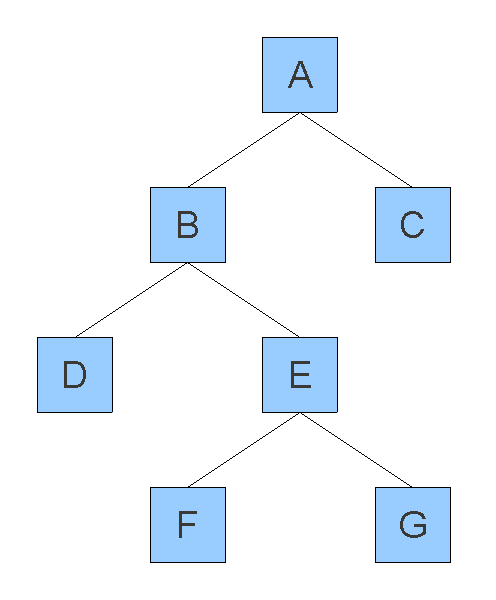
\includegraphics[width = 3.00in]{splittingTree}}
\caption{Splitting Binary Tree: Node A is the root, B and E are internal nodes, and C, D,  F, and G are leaves.  Notice how all internal nodes have degree $3$.}
\end{figure}


\begin{figure}[p]
\label{binary}
\centerline{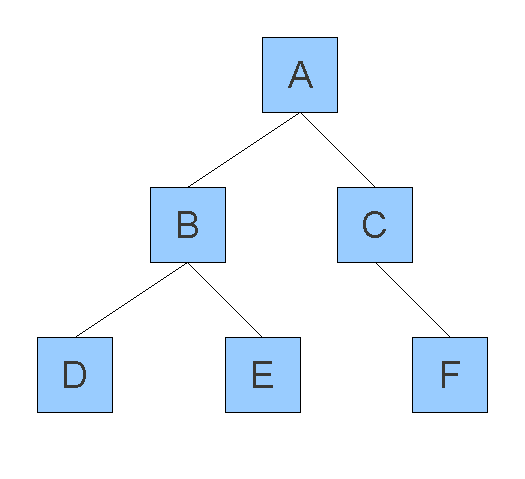
\includegraphics[width = 3.00in]{binaryTree}}
\caption{This is an example of a tree which is NOT a Splitting Binary Tree.  Notice how both A and C have degree $2$, when a BSTree can only have one such node.}
\end{figure}

\bparts

\ppart {10} Show if an SBTree has more than one vertex, then the induced subgraph obtained by removing the unique root consists of two disconnected SBTrees. You may assume that by removing the root you obtain two separate connected componenents, so all you need to prove is that those two components are SBTrees.

\solution{ 
Consider one of the two connected components. We must show it is:

\begin{enumerate}
\item Connected: we get this for free because this is a connected component.
\item Acyclic: suppose there is a cycle in our component. Since this component is a subgraph of the original SBTree, then the original SBTree would have had a cycle.
\item SBTrees: by showing it is connected and acyclic, we have checked it is a tree. Now it remains to show it is also an SBTree. We have two cases to consider. Perhaps the node connected to the root (in our connected component) had degree 1 originally, in which case the full connected component is a lone vertex, and hence an SBTree.  Otherwise, the node was of degree 3 originally, so it is now a degree 2 node. Any other remaining node in the connected component would have its degree intact, so it must be of degree 3 or 1. Hence the connected component is an SBTree.
\end{enumerate}
}

\ppart {10} Prove that two SBTrees with the same number of leaves must also have the same total number of nodes. \emph{Hint: As a conjecture, guess an expression for the total number of nodes in terms of the number of leaves $N\left(l\right)$.  Then use induction to prove that it holds for all trees with the same \( l \).\\}

\solution{ 
You can deduce a formula by experimentation. Our guess is  \( N\left(l\right) = 2l - 1 \). 

\begin{proof}
We will now verify this formula by strong induction on $l$, the number of leaves. 

\begin{enumerate}
\item  Base case:
  If $l = 1$ Then we have one leaf, hence this is the sinlge vertex SBTree. So the total number of nodes is \( 1 \) which agrees with our formula: \( 2\cdot 1 - 1 \).

\item Induction step:

  Assume that for all \(1 \leq l \leq k\), an SBTree with \( l \) leaves in it has \( 2l - 1 \) nodes in total, regardless of its particular structure. We wish to prove that every SBTree of size \( k + 1 \) has \(2 \left(k + 1 \right) - 1\) nodes in total. Consider a generic SBTree with \(k + 1 \) leaves. We assume \(k\) is greater than or equal to 1, so our graph has two subgraphs connected to a root. From the first part we know each is an SBTree. 

  We cannot assume anything about their structure, but we know  if denote by \( \ll \) the  number of leaves in the left child, and by \( \lr \) the number of leaves in the right side then we must have \( k + 1 = \ll + \lr \). And also, \( 0 < \ll\mbox{, } \lr < k + 1 \). Hence, by our induction hypothesis, the number of nodes in the left is \( N \left(  \ll \right)  = 2\ll - 1 \) and the number of nodes in the right is \(N \left( \lr \right) = 2\lr - 1\). And the total number of nodes in the tree must be \(N \left(\lr \right) + N(\ll) + 1\), accounting for the root. Substituting, we get \( 2\lr - 1 + 2\ll - 1  + 1 = 2(\lr + \ll) - 1 = 2(k+1) - 1 \), as we wanted to show.
\end{enumerate}
\end{proof}
}
\eparts

\end{problem}

\end{comment}

%%%%%%%%%%%%%%%%%%%%%%%%%%%%%%%%%%%%%%%%%%%%%%%%%%%%%%%%%%%%%%%%%%%%%%%%%%%

\begin{problem}{15}
%topics: hamiltonian cycles, two coloring - bipartite, induction

In "Die Hard: The Afterlife", the ghosts of Bruce and Sam have been
sent by the evil Simon on another mission to save  midtown
Manhattan. They have been told that there is a bomb on a street
corner that lies in Midtown Manhattan, which Simon defines as
extending from 41st Street to 59th Street and from 3rd Avenue to 9th
Avenue. Additionally, the code that they need to defuse the bomb is
on another street corner. Simon, in a good mood, also tosses them
two carrots:

\begin{itemize}
\item He will have a helicopter that initially lowers them to the street corner where the bomb is.
\item He promises that the code is placed only on a corner of a numbered
street and a numbered avenue, so they don't have to search Broadway.
\end{itemize}

The map of midtown Manhattan is an example of an $N \times M$
(undirected) grid.  In particular, midtown Manhattan is a $19 \times
7$ grid.

%INSERT FIGURE of 19 by 7 grid

Bruce and Sam need to check all $19 \cdot 7 = 133$ street corners
for the code.  Once they are at a corner, they don't need any
additional time to verify whether the code is there.  Once they find the
code and return to the bomb, they can disarm it in 2 minutes (even,
or especially, as the timer ticks down to 0). Also, they can run one
block (in any of the four directions) in exactly 1 minute.
%(even though avenue blocks are longer than
%street blocks in NYC, it takes them the same amount of time for each
%kind).
They are given 135 minutes total to find the code and
disarm the bomb, which means that they need to return to the bomb,
code in hand, in 133 minutes.

Sam realizes that the map of NYC is actually a graph, and that they
need to use a cool new 6.042 concept: a {\em Hamiltonian cycle} is a
path that visits each vertex in a graph exactly once and ends at its
starting point (so it is a cycle). A graph is {\em Hamiltonian} if
it has a Hamiltonian cycle.

Hamiltonian graphs are really useful because you can visit each node
and return to the starting point by taking only $n$ steps, where $n$
is the number of nodes -- if a graph is not Hamiltonian, you would
need at least $n+1$ steps to visit each of the $n$ nodes and return
to the starting point.

In general, we don't know how to efficiently determine whether a
general graph is Hamiltonian. However, Sam is very excited
because he thinks he can show that Midtown Manhattan is
Hamiltonian.  If it is, Bruce and Sam can save the day! Will they
make it?

\bparts

\ppart {6} Show that they cannot do it -- that is, more generally,
show that if both $N$ and $M$ are odd, then the $N\times M$
grid is {\em not} Hamiltonian. {\em Hint:
First show that any $N \times M$ 2-dimensional undirected grid is
bipartite.}
\solution{ Any 2-dimensional undirected grid is bipartite. To show this fact, let us exhibit a coloring of such grid with 2 colors $\{0,1\}$: 
indexing the vertices of the grid by their $(x,y)$-coordinates and then coloring vertex $(i,j)$ with color $rem(i+j, 2)$. The resulting colored grid now has each vertex adjacent to only vertices in the other color.  Since any connected graph that can be colored by two distinct colors is bipartite, any $N \times M$ 2-dimensional undirected grid is bipartite.

Suppose the $N \times M$ grid is Hamiltonian. Since $N$ and $M$ are both odd, there is an odd number of vertices in the 
grid. It follows that the Hamiltonian cycle in this grid is an odd cycle. However, since we have already shown that any 2-dimensional undirected grid is bipartite, odd cycles are not possible.  We have reached a contradiction; thus, our supposition that the grid was Hamiltonian is wrong, and we are done.
}

\ppart {9}
Suppose Simon defined Midtown in the more standard way
as extending from 40th Street to 59th Street and from 3rd Avenue to 9th
Avenue (that is suppose Midtown Manhattan was a $20 \times 7$ grid),
and gave them another 7 minutes,
\begin{enumerate}
\item
Show that if either $N$  is  even and $M > 1$ or  $M$ is even and $N > 1$, then the $N\times M$ grid is Hamiltonian.
\solution{Suppose $N$ is even (WLOG).  We can write a direct proof or an inductive proof.

Direct constructive proof:

Assume the grid is laid out on the plane occupying the integer points 
between $(0,0)$ and $(N-1, M-1)$.

We find the Hamiltonian path explicitly by specifying the $k$'th 
vertex visited for each $k$ from $0$ to $NM$. Let $q = \lfloor 
\frac{k}{M-1} \rfloor$ and let $r = rem(k, M-1)$.

On step $k$:
\begin{itemize}
\item if $k \leq N(M-1)$ and $q$ is even, then visit vertex $(q,r+1)$.
\item if $k \leq N(M-1)$ and $q$ is odd, then visit vertex $(q, M-1-r)$.
\item if $k > N(M-1)$, then visit vertex $(0,N - (k-N(M-1)))$.
\end{itemize}

Checking that it is a Hamiltonian cycle is routine.

Figure $2$ shows a picture of such a cycle.\\

\begin{figure}[p]
\label{hamcy}
\centerline{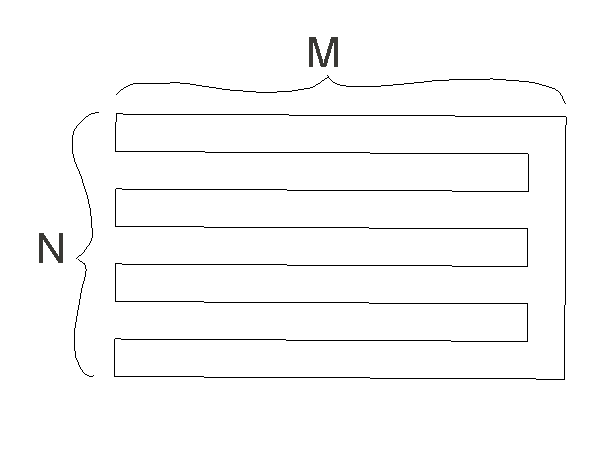
\includegraphics[width = 3.00in]{hamCycle}}
\caption{Hamiltonian cycle described in solution for 2b.}
\end{figure}

Inductive proof (also constructive):\\
We induct on even$ N$ values.  For the base case $N=2$, our cycle just has all the exterior edges of the grid.\\
For the inductive step, we assume the existence of a Ham-cycle $H$ on an $N \times M$ grid, and construct a Ham-cycle on the $N+2,M$ grid.  Then, consider vertex $v=(n-1,0)$ (this is at one 'corner' of the grid).  By def. of Ham-cycle, $H$ must include $v$, and thus $v$ must 2 distinct edges incident.  There are only 2 such edges possible on the grid, and it follows that the edge $((n-1,0),(n-1,1))$ is in $H$.  We can remove that edge and add edges $((n-1,0),(n,0))$, $((n,0),(n+1,0))$, $((n,i),(n,i+1)$ for $1\le i <m$, $((n+1,i),(n+1,i+1))$ for $0 \le i < m$, and $((n,m-1),(n+1,m-1))$.  See Figure $3$.

\begin{figure}[p]
\label{hamind}
\centerline{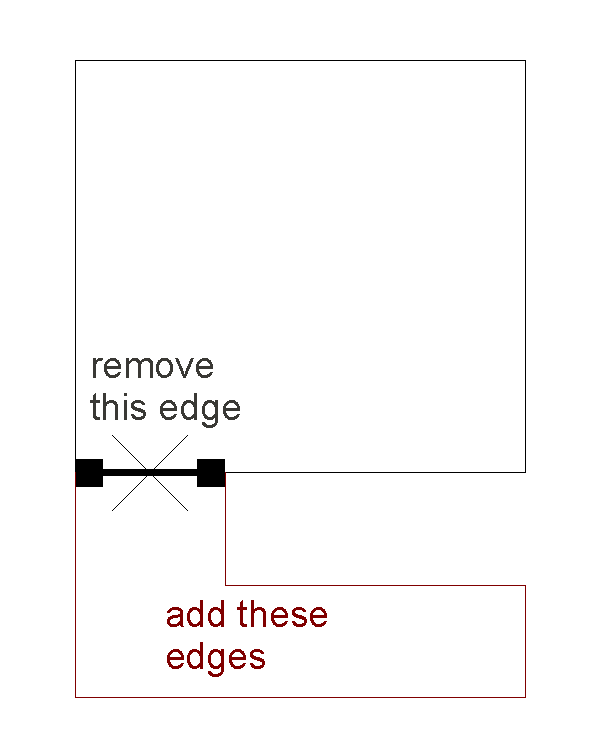
\includegraphics[width = 3.00in]{p2induction}}
\caption{Inductive step for existence of Hamiltonian cycle.}
\end{figure}
}

\item Explain why your proof breaks down when $N$ and $M$ are odd.
\solution{ For the direct proof, the odd/even conditions on $q$ require $N$ to be even 
for the above sequence of vertices to actually form a cycle.  For the inductive proof, note that the base case depends on $N$ being $2$.

}
\item
Would they survive? Does the outcome depend on where the bomb is placed?
\solution{Come on, Bruce and Sam would survive, of course!  Their survival doesn't depend on where the bomb is 
placed!
}
\end{enumerate}

\eparts
\end{problem}

%%%%%%%%%%%%%%%%%%%%%%%%%%%%%%%%%%%%%%%%
%%%%%%%%%%%%%%%%%%%%%%%%%%%%%%%%%%%%%%%%
% New problem
\vspace{12pt}

\begin{problem}{10} 
Let the nodes in a tournament be ranked
according to their outdegrees, that is, node $u$ is ranked less than or equal to $v$ iff $outdegree(u)\leq outdegree(v)$.
Prove that the sum of the
outdegrees of the $i$ lowest ranked nodes is at least $i(i-1)/2$.\\

\solution{
Consider the subgraph on the $i$ lowest ranked nodes. This subgraph represents a
tournament as well (see the inductive step in the proof for Theorem 6.2.1 in the textbook).  Thus, there is exactly one directed edge between every pair of distinct vertices $1, 2,...,i$, and the number of edges in the subgraph is equal to $i(i-1)/2$. Each of these edges are counted in the sum of the outdegrees of these $i$ nodes in the original graph; it follows that the sum of the outdegrees of the $i$ lowest ranked nodes in the original tournament is at least $i(i-1)/2$.

}
\end{problem}
%\instatements{\vspace{0.3in}}

%%%%%%%%%%%%%%%%%%%%%%%%%%%%%%%%%%%%%%%%
%%%%%%%%%%%%%%%%%%%%%%%%%%%%%%%%%%%%%%%%
% New problem

\begin{comment}
\begin{problem}{12}

%In lecture, we discussed the notion of 
We can pair up boys and girls by finding a \textit{minimum weight matching} on the bipartite graph $G$, where the weight of an edge $b$---$g$ is the sum of the rank of the $g$ on $b$'s list plus the rank of $b$ on $g$'s list. The minimum weight matching of $G$ is the matching that produces the lowest sum of weights on the edges of $G$.

\textbf{Ex.} If boy $b_1$ has a ranking of girls $g_1,g_2,g_3,g_4$, and girl $g_1$ has a ranking of boys $b_2,b_3,b_4,b_1$, then the weight of the edge $b_1$---$g_1$ will be $1+4 = 5$, since $g_1$ is ranked first and $b_1$ is ranked fourth.

\begin{problemparts}

\ppart {6}
Prove that the minimum weight matching is not always a stable matching by providing a counterexample.

\textit{(Hint: There is a counterexample with 3 boys and 3 girls.)}

\solution{Consider the counterexample shown below. The minimum weight matching gives a sum of weights $3+3+4 = 10$. However, there is a rogue couple between B2 and G2 (shown in the dotted line), who prefer each other to their mates.

\begin{figure}[htbp]
\centerline{\includegraphics[width=4in]{minweightmatch}}
\end{figure}
}

\ppart {6}
The minimum weight matching minimizes the sum over \textit{all} possible matchings. Instead, consider a greedy algorithm that recursively matches the minimum weight edge over all unmatched nodes. Prove that this matching is also not always a stable matching by providing a counterexample.

\textbf{Ex.} If all boys have the same ranking of girls $g_1,g_2,g_3,g_4$, and all girls have the same ranking of boys $b_1,b_2,b_3,b_4$, then $b_1$---$g_1$ will be matched first (weight$=2$), $b_2$---$g_2$ will be matched second (weight$=4$), $b_3$---$g_3$ will be matched third (weight$=6$), and $b_4$---$g_4$ will be matched last (weight$=8$).

Note two things:
\begin{itemize}
\item Suppose that, in the case of a tie for minimum weight edge, the algorithm matches all of the tied edges. If this creates a conflict (for example, if $g_1$---$b_1$ and $g_1$---$b_2$ both have weight$=3$), then the algorithm just matches one of the pairs randomly (for example, $g_1$---$b_1$). Choose a counterexample with no such conflict.
\item The algorithm does \textit{not} recalculate the weights after each recursion, so the weight of an edge does not change, even as higher ranked preferences become unavailable. There is also a counterexample to stability for such an algorithm that does reweight the edges, but it's much more difficult to find!
\end{itemize}

\textit{(Hint: There is a counterexample with 4 boys and 4 girls.)\\}

\solution{Consider the counterexample shown below. The first round of the algorithm removes the edges B3--G3 and B4--G4, which both have weights of 2. The second round pairs up B1--G2 and B2---G1, which each have weight of 5, less than the weight 8 of B1---G1 and weight 6 of B2---G2. However, there is a rogue couple between B2 and G2 (shown in the dotted line), who prefer each other to their mates.

\begin{figure}[htbp]
\centerline{\includegraphics[width=4in]{minweightmatch2}}
\end{figure}
}

\end{problemparts}

\end{problem}
\end{comment}

%\instatements{\newpage}

%\newpage
%%%%%%%%%%%%%%%%%%%%%%%%%%%%%%%%%%%%%%%%
%%%%%%%%%%%%%%%%%%%%%%%%%%%%%%%%%%%%%%%%

\begin{problem}{16}
\begin{problemparts}

\ppart{8}
%Suppose that $G$ is a simple, connected graph on $n$ nodes. Show that $G$ has exactly $n-1$ edges if $G$ is a tree.
Prove that a simple connected graph with $n$ nodes and $n-1$ edges is a tree.
\solution{
%To show the biimplication, it is necessary to show both that if $G$ is a tree then it has $n-1$ edges \emph{and also} if $G$ has $n-1$ edges then it is a tree. The first part was proved in lecture by induction on the number of nodes. We prove the second part by contradiction.

To show that a connected graph $G$ with $n$ nodes and $n-1$ edges is a tree, it is sufficient to show that it is acyclic. Assume to the contrary that there is a cycle in $G$. We can remove the edge in this cycle that preserves connectivity, and continue to remove edges from $G$ until the resulting subgraph no longer contains a cycle; effectively, we are forming a connected acyclic graph $G'$. $G'$ is by definition a tree, but it has fewer than $n-1$ edges since we removed at least one edge from $G$; thus, we have reached a contradition and conclude that a simple connected graph with $n$ nodes and $n-1$ edges is a tree.
}

\ppart{8}
Prove by induction that any connected graph has a spanning tree.

\solution{
The proof is by induction on the number of edges. Let P(k) be the predicate that if $G$ is connected with $k \geq n-1$ edges, then $G$ has a spanning tree.

\textbf{Base Case}: $k = n - 1$. Part (a) demonstrates that $G$ is a tree and thus a spanning tree of itself.

\textbf{Inductive Step}: Assume P(k). If $G$ is a connected graph with $k+1 > n-1$ edges, it must not be a tree, by Part (a).  It follows that $G$ must have a cycle.  Removing an edge from that cycle creates a connected graph $G'$ with $k$ edges, which has a spanning tree over the nodes by our inductive hypothesis.  This spanning tree is also a spanning tree over $G$, thus P($k+1$) holds.

By induction, a connected graph $G$ with $k$ edges has a spanning tree, for all $k \geq n - 1$. 

} 
\end{problemparts}

\end{problem}
%\instatements{\vspace{0.3in}}

%%%%%%%%%%%%%%%%%%%%%%%%%%%%%%%%%%%%%%%%
%%%%%%%%%%%%%%%%%%%%%%%%%%%%%%%%%%%%%%%%

\begin{comment}
% From Spring08, Pset6
\begin{problem}{15}

  A $3$-bit string is a string made up of $3$ characters, each a $0$
  or a $1$.  Suppose you'd like to write out, in one string, all eight
  of the 3-bit strings in any convenient order.  For example, if you
  wrote out the $3$-bit strings in the usual order starting with
  000 001 010\dots, you could concatenate them together to get a
  length $3\cdot 8 = 24$ string that started 000001010\dots.

  But you can get a shorter string containing all eight $3$-bit
  strings by starting with 00010\dots.  Now $000$ is present as bits
  $1$ through $3$, $001$ is present as bits $2$ through $4$, $010$ is
  present as bits $3$ through $5$, \dots.

\bparts

\ppart {3} Take a few moments to see how short a string you can make that
contains every $3$-bit string as $3$ consecutive bits somewhere in it.
Explain why $10$ bits is the absolute minimum length for such a
string.

\solution{$0001110100$ does it with $10$ bits and you can't do better:
  there must be two bits to start and each additional bit can yield at
  most one new $3$-bit string.}

\begin{figure} [htbp]
\centerline{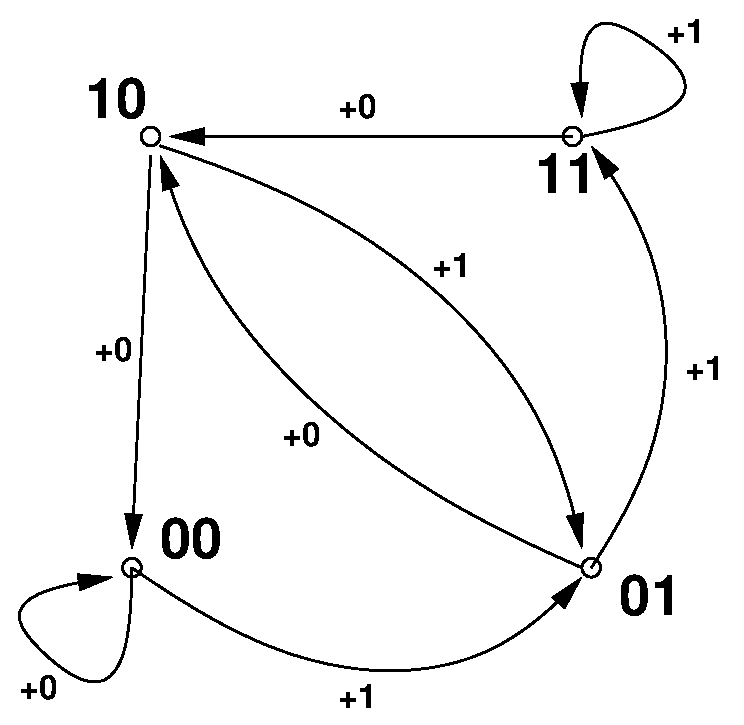
\includegraphics[width=2in]{debruijn}}
\end{figure}

\ppart {3} Imagine that the labels on the vertices of the directed graph above
represent the last two digits in a string you build by adding one bit
at a time.  Explain why the graph completely describes how
the last two digits of your string can change throughout this process.

\solution{No matter what the last two bits of your current string $x$
  are, say $ab$, there is a vertex representing that.  And, no matter
  what bit you want to use to extend $x$, say $c$, there is an edge
  directed from your current state, $ab$, to the vertex $bc$ that
  represents your new state, the last two bits of $xc$.  Furthermore,
  these are the only types of vertices and edges in the graph.  As a
  bonus, every edge $(s,s')$ is also labeled with the bit that was
  added to the string when going from the state $s$ to $s'$.}

\ppart {3} Find a directed path in this graph starting at some vertex, $v$,
that traverses every edge exactly once.  Note that vertices will have to
be used more than once and the path wil have to end in $v$.

\solution{Many: $00,00,01,11,11,10,01,10,00$ is one.}

\ppart {3} Explain how such a path provides a shortest possible solution
to the original problem.

\solution{Build a solution $x$ using the path.  Start with $x$ equal
  to the two digits in the label of the first vertex on the path.
  Then for every edge used after that, add on the bit labelling that
  edge to the string.  For example, the path given in last part's
  solution, yields the string $x=0001110100$.
  
  Since there are $8$ edges, the string will be of length $10$, the
  minimum possible.

  Furthermore, the label of the first vertex of the graph, followed by
  the label of the first edge, give the first $3$-bit substring in
  $x$. The next vertex and edge, give the next $3$-bit substring, and
  so on.  Since all possible $2$-bit vertex labels appear exactly
  once, and each vertex has a $1$ edge and a $0$ edge departing from
  it, every $3$-bit string corresponds to a unique vertex/out-edge
  combination.  The path uses every possible vertex/out-edge
  combination exactly once, so the string contains every $3$-bit
  sequence exactly once.}

\ppart  {3} What about $k$-bit substrings, $k = 4, 5, \ldots$?  Can you define the appropriate
generalization of the useful graph above?  (They're called de Bruijn
graphs.) If you do it sucessfully, you should be able to see that the
in-degree (as well as the out-degree) of every vertex is $2$.

\solution{
There are $2^k$ possible $k$-bit substrings. We can create $2^{k-1}$ nodes representing the different possible combinations of the first $k-1$ bits. The last bit will be represented as two edges out of each node (0 or 1) and two edges into each node (0 or 1).

It is a theorem that if the in-degree is equal to the out-degree at
every vertex of a digraph (and if the graph is connected when all the
edges are considered undirected edges) then a directed path can be
drawn in that digraph that uses every edge exactly once.  You might
want to think about why this should be true or how you might find such
a path.

But if you do believe it, you should be able to see why all $2^k$
$k$-bit strings can be written as substrings of a string of length
$2^k + k-1$.  (These strings are essentially de Bruijn strings.)}

\eparts

\end{problem}
\end{comment}

%%%%%%%%%%%%%%%%%%%%%%%%%%%%%%%%%%%%%%%%%%%%%%%%%

\begin{problem}{10}

Show that the congestion of the $N$-input butterfly is $\sqrt{N}$ if $N$ is an even power of 2.

\solution{
First we will show that the congestion is at most  $\sqrt{N}$.

Let $v$ be an arbitrary vertex at some level $i$. Let $S_v$ be the
set of inputs that can reach vertex $v$. Let $T_v$ be the set of
outputs that are reachable from vertex $v$.

Note that:
\begin{itemize}
\item For the butterfly network, there is a unique path from
each input to each output, so the congestion is the maximum number
of messages passing through a vertex for any matching of inputs to
outputs.
\item If $v$ is a vertex at level $i$ of the butterfly
network, there is a path from exactly $2^i$ input vertices to $v$
and a path from $v$ to exactly $2^{n-i}$ output vertices.\\
\end{itemize}

We thus have $\card{S_v} = 2^i$ and $\card{T_v} = 2^{n-i}$.
The number of inputs in $S_v$ that are matched with outputs in $T_v$
is at most $\min \set{2^i,2^{n-i}}$.  To obtain an upper-bound on
the congestion of the network, we need to find the maximum value of
$\min \set{2^i,2^{n-i}}$, where the maximum is taken over all $i$.
The maximum value is achieved when $2^i$ and $2^{n-i}$ are as equal
as possible. Since $n$ is even, these two quantities are equal when
$i=n/2$, hence the maximum congestion is
$2^{n/2}=N^{1/2} = \sqrt{N}$.


So far, we have concluded that the congestion of
$\sqrt{N}$ can be achieved only at a node at level $\frac{n}{2}$.
Now consider the node at that level whose binary representation is all
$0$s. Any packet from the input in the form
$z\underbrace{0\ldots000}_{n/2\ bits}$ with destination
$\underbrace{000\ldots0}_{n/2\ bits}z'$, where $z$ and $z'$ are any
$\frac{n}{2}$-bit numbers, must pass through this node. In the worse case, all packets from  input in the form
$z\underbrace{0\ldots000}_{n/2\ bits}$ will have destination in the form
$\underbrace{000\ldots0}_{n/2\ bits}z'$.  But there
are $2^{n/2}=\sqrt{N}$ of such possible packets, giving the node load $\sqrt{N}$.
Therefore, we can conclude that the congestion of $B_n$ is exactly
$\sqrt{N}$ when $n$ is even.

}
\end{problem}

%%%%%%%%%%%%%%%%%%%%%%%%%%%%%%%%%%%%%%%%%%%%%%%%%


\begin{problem}{20} 

In a \emph{perfect shuffle}, a deck of $N$ cards is cut exactly in half and then perfectly interlaced. Thus, for $N$ cards, we would obtain the resulting cards in the following order:\\ $1, (\frac{N}{2}+1), 2, (\frac{N}{2}+2), ..., (\frac{N}{2}-1), (N-1), (\frac{N}{2}), N$. 


\bparts

\ppart{10} Show that $m$ perfect shuffles will return a deck of $N$ cards to its original order provided that $2^m \equiv 1 \pmod{(N-1)}$.

\solution{Let $N \times m$ switches $P_{0}^{1}, P_{1}^{1},..., P_{N-1}^{m}$  be available, where $N=2^{m}$ for some positive interger $m$.  In this network of $N \times m$ switches, there is a one-way link connecting $P_{i}$ to $P_{j}$, where $j=2i$ for $0 \leq i \leq N/2-1$ and $j=2i+i-N$ for $N/2 \leq i \leq N-1$.

Now, let the binary representation of $i$ be $b_{m-1}b_{m-2}...b_{1}b_{0}$, where $b_{k}=0$  or $1$, for $0 \leq k \leq m-1$.  Then, the binary representation of $j$ be $b_{m-2}b_{m-3}...b_{0}b_{m-1}$,  where $b_{k}=0$ or $1$, for $0 \leq k \leq m-1$; such that,

\centerline{$i=b_{m-1}2^{m-1}+b_{m-2}2^{m-2}+...+b_{1}2+b_{0}$}
\centerline{$j=b_{m-2}2^{m-1}+b_{m-3}2^{m-2}+...+b_{0}2+b_{m-1}$}

We see that the binary representation of $j$ is obtained by cyclically shifting the binary representation of $i$ one position to the right.  For example, when $m=3$, we have

\newpage

\begin{figure}[h]
\label{tentree}
\centerline{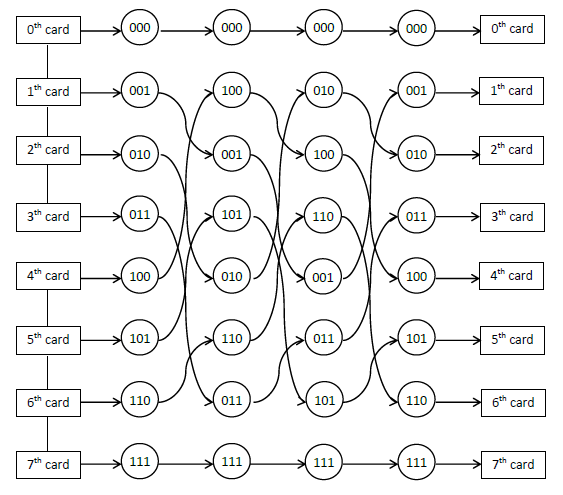
\includegraphics[scale=1]{ps5_fig4t.png}}
\caption{Switch Network for $m=3$ Perfect Shuffles}
\end{figure}

\vspace{18pt}
\centerline{$000 \to 000,   001 \to 100,   010 \to 001,   011 \to 101$}
\centerline{$100 \to 010, 101 \to 110, 110 \to 011, 111 \to 111$}
\vspace{18pt}


We see in Figure 4, where each of the eight cards is represented by a 3-digit binary sequence, this deck of cards is returned to its original order after 3 perfect shuffles.

Since  $2^m \equiv 1 \pmod{(N-1)}$, we could map $m$ applications of the perfect-shuffle onto a network of $m$ columns of $N$ switches, interconnected by the one-way link described earlier.  Given that each binary digit of the input data returns to its original position at the output, $m$ perfect shuffles will return a deck of $N$ cards to its original order.

\emph{Another approach to this problem:} Let us first identify a pattern in how $N$ cards shift during a perfect shuffle. We have two sets of cards that are produced from the cut; let's call them sets T and B: T represents the top set/half of cards, and B the bottom set/half. Note that the first card of set T is the original $0^{th}$-position card, and the first card of set B is the formerly $(N/2)^{th}$-position card. For the sake of simplicity of our future formulation, let us assume that the first card after the first perfect shuffle comes from set T (i.e., the $0^{th}$ card).
 
The cards in set T were originally indexed 0 through $(N/2 - 1)$.  After the perfect shuffle, card $i$ will end up in position $2i$ (all the even positions). The cards in set B were originally indexed $N/2$ through $(N - 1)$, and each card $i$ will end up in position $2(i - N/2) + 1$ (all the odd positions). For easy mapping, we now index both T and B starting with 0: for set T, $(0, 1, 2, 3, ...) \to (0, 2, 4, 6, ...)$, and for set B, $(0, 1, 2, 3, ...) \to (1, 3, 5, 7, ...)$. Now we need to be able to re-index $N/2$ through $(N - 1)$ down to 0 through $(N/2 - 1)$, which could be achieved by subtracting off $N/2$. Hence we replace $i$ with $(i - N/2)$ to get $2(i - N/2) + 1$.
 
We can rewrite $2(i - N/2) + 1$ as $2i - N + 1$ and then as $2i - (N - 1)$. Essentially, all cards, regardless of being in T or B, will be mapped as $i \to rem(2i, N - 1)$: $N - 1$ comes from the fact that the bottom card, the $(N - 1)^{th}$-position card, never moves during the shuffle. Note that the $0^{th}$-position card never moves either, as reflected by the mapping $2 \times 0 = 0$.
 
Bringing the above mappings and derivations together, the position of card $i$ after $m$ shuffles will be $rem(i \times 2^m, N - 1)$. This can be rewritten as $i  \times 2^m \equiv r  (mod (N - 1))$, where r is the resulting position of the card. However, we are supplied with $2^m \equiv 1
 (mod (N - 1))$, so we can multiply each side by $i$ to get $i \times 2^m \equiv i (mod (N - 1))$, which means that $r = i$. Therefore, we conclude that since $ i \times 2^m \equiv i (mod (N - 1))$, after $ m$ shuffles, card $i$ will be back to its original position.

}

\ppart{4} Show that 8 perfect shuffles are necessary and sufficient to return a deck of 52 cards to their original order.

\solution{Substituting 8 for $m$ and 52 for $N$, where $m$ and $N$ are related as in Part (a), we find from the congurence below that 8 perfect shuffles are sufficient to return a deck of 52 cards to their original order. 

\centerline{$2^m \equiv 1 \pmod{(N-1)}$}

\centerline{$2^8 \equiv 1 \pmod{(52-1)}$}

\centerline{$256 \equiv 1 \pmod{51}$}

\centerline{$\frac{256-1}{51} = 5$ }


We also note that $2^m \not\equiv 1 \pmod{(N-1)}$ for $N=52$ and $1 \leq m < 8$.  Therefore, 8 perfect shuffles are necessary to return a deck of 52 cards to their original order.


 
}

\ppart{6} How many perfect shuffles are necessary and sufficient to return a deck of cards to its original order if there are two jokers added to the deck (so that it has 54 cards)?

\solution{52. Note that the top and bottom cards never move.  Consider a card $C$
with $i \in \set{1, 2, \ldots, 52}$ cards above.  After 52 perfect shuffles:
\begin{eqnarray*}
\text{\# of cards above $C$}
    & \equiv & 2^{52} \cdot i \pmod{53} \\
    & \equiv & 1 \cdot i \pmod{53} \\
    & \equiv & i \pmod{53}
\end{eqnarray*}

The second congruence uses Fermat's Theorem, which implies that
$2^{52} \equiv 1 \pmod{53}$.  If the number of cards above $C$ is
congruent to $i \in \set{1, 2, \ldots, 52}$, then it must be equal to $i$.  Thus, every card returns to its original position and the deck
is restored after 52 perfect shuffles.

}

\eparts

\end{problem}

%%%%%%%%%%%%%%%%%%%%%%%%%%%%%%%%%%%%%%%%%%%%%%%%%
%newpage

\begin{problem}{10}

For the \emph{Grid, Interrupted} switching network, find the diameter and congestion. Give a reason for your answer. \\

\begin{figure}[h]
\label{tentree}
\centerline{\includegraphics[scale=0.85]{ps5_fig2new2t.pdf}}
\caption{Grid, Interrupted}
\end{figure}

\solution{
Diameter is 16.  Input $in_{0}$ and output $out_{4}$ are farthest apart, and the shortest path between the two has a distance of 16.

Congestion is 3.  The maximum congestion that will be ever suffered by switches with the most inputs is 3.    

}

\end{problem}

%%%%%%%%%%%%%%%%%%%%%%%%%%%%%%%%%%%%%%%%%%%%%%%%%

\begin{problem}{10}

Construct a 16-bit de Bruijn sequence.

\solution{ 

We can construct a 16-bit de Bruijn sequence using the labels on the edges of an Euler tour in the de Bruijn graph (see Lecture 9 handout): 0111100101000011.

}

\end{problem}

%%%%%%%%%%%%%%%%%%%%%%%%%%%%%%%%%%%%%%%%%%%%%%%%%


\end{document}
